\section{Black Pepper}
\label{sec:pepper}

\begin{spice}\label{spice:pepper}
\textsc{Pepper} \hfill \href{https://powo.science.kew.org/taxon/682369-1}{POWO} \\
\textbf{English:} \textit{pepper}; \textit{black pepper}. 
\textbf{Arabic:} {\arabicfont{فلفل}} \textit{filfil, fulful}. 
\textbf{Chinese:} {\tradchinesefont{胡椒}} \textit{hújiāo} [foreign-pepper]; 黑胡椒 \textit{hēihújiāo} [black-barbarian-pepper]. 
\textbf{Hungarian:} \textit{bors}; \textit{fekete bors} [black pepper].  \\
\noindent{\color{black}\rule[0.5ex]{\linewidth}{.5pt}}
\begin{tabular}{@{}p{0.25\linewidth}@{}p{0.75\linewidth}@{}}
Plant species: & \taxonn{Piper nigrum}{L.} \\
Family: & \textit{Piperaceae} \\
Plant part used: & fruit \\
Region of origin: & Malabar coast (South India) \\
Cultivated in: & Vietnam; Brazil; Indonesia; India; Sri Lanka; etc. \\
Color: & black; white; green \\
\end{tabular}
\end{spice}

\begin{figure}[!ht]
	\vspace{-4ex}
	\centering
	\subfloat{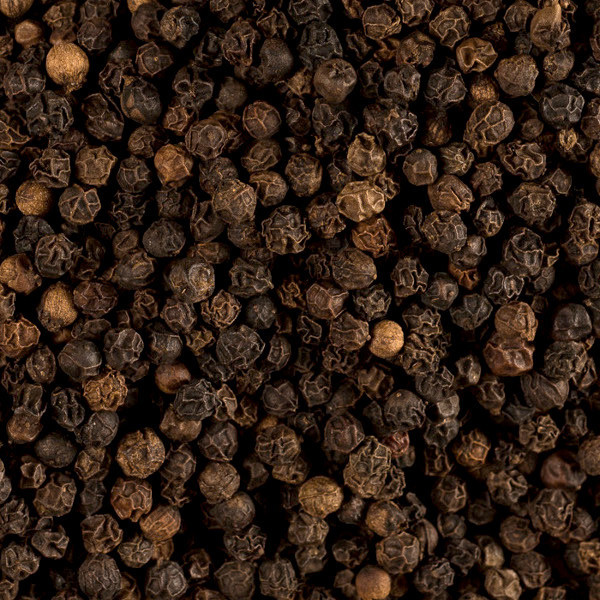
\includegraphics[width=0.3\linewidth]{imgs/spices/pepper-black-2.jpg}}
	\hfill
	\subfloat{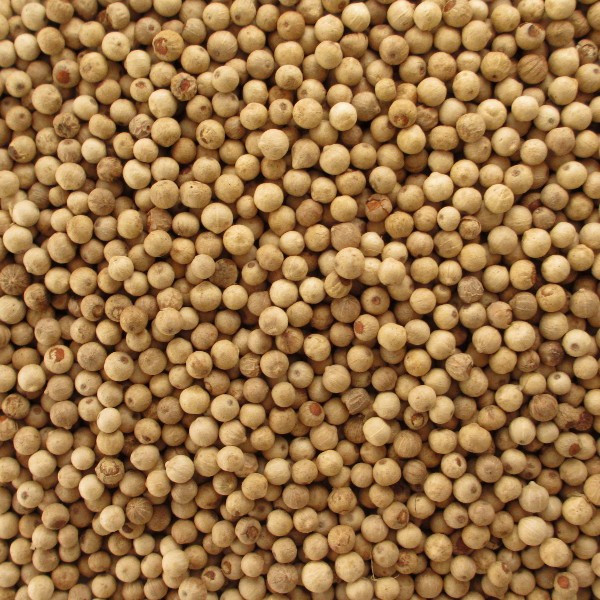
\includegraphics[width=0.3\linewidth]{imgs/spices/pepper-white-penja-2.jpg}}
	\hfill
	\subfloat{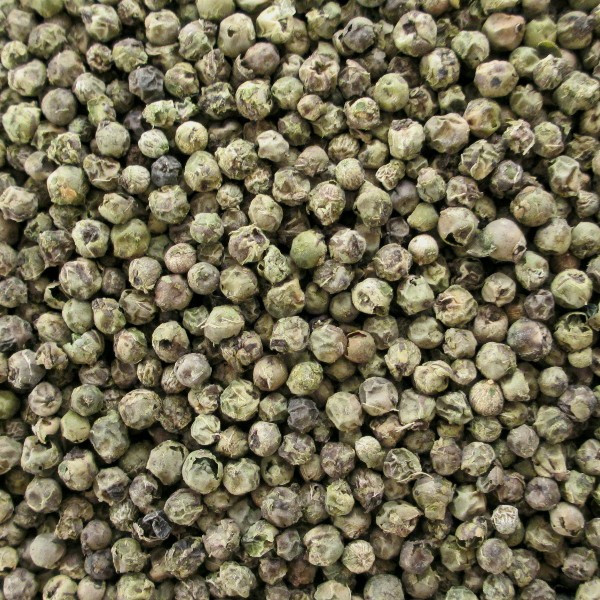
\includegraphics[width=0.3\linewidth]{imgs/spices/pepper-green-1.jpg}}
	\caption[Black, white, and green pepper.]{Black pepper from the Malabar coast in India, white pepper from the Penja Valley in Cameroon, and green peppercorns. \taxon{Piper nigrum}. Credits: Aromatiques.}
	\label{fig:pepper_imgs}
\end{figure}

% DESCRIPTION:
Black pepper is the dried fruit (drupe)\footnote{A type of fleshy fruit with thin skin and a single, central pit containing the seed, also known as a ``stone-fruit'' (e.g.: plum, cherry, peach, nutmeg, olive, mango). It is a term used to denote the contrast to a botanical ``berry'', which contains many seeds (e.g.: blueberry, grape).} of the species \taxon{Piper nigrum}. Pepper fruits are often called peppercorns, and they come in black, white, green, and even red. However, black pepper\index{pepper!black}, white pepper\index{pepper!white}, green\index{pepper!green} and ``true'' red peppercorns\index{pepper!red} are not different varieties, they are the fruits of the same plant. Their difference merely lies in the harvesting and drying process. All of them have a unique, pungent taste and a fresh, spicy aroma that they release when being crushed or ground. 

% INTRO:
Black pepper\index{pepper|textbf}\index{pepper!black} is the most important, most popular, and most consumed spice in the world \autocite[721]{mabberley_mabberleys_2017}. Valued for its pungency and flavor, pepper has been used since ancient times in traditional medicine and gastronomy from East to West, and it is the most influential spice that shaped human history. It is found and used virtually everywhere around the globe \autocite[253]{hill_contemporary_2004}, and most of us are familiar with the biting sensation it causes on the tongue and in the nose. Black pepper was one of the first aromatic substances used medicinally in India, and one of the first products of global commerce to be traded, alongside long pepper, and ginger. It was transplanted to other tropical regions of Asia early on, and cultivated extensively. Black pepper's early diffusion is remarkably interesting, it is the prototype spice for many of us. Also referred to simply as \textit{pepper} from here on, it was among the first oriental spices to reach the Occident \pvolcite[]{1}[86]{peter_handbook_2012}. Pepper was known to the ancient Egyptians, Greeks, and Romans in the West, and have changed medieval Europe. It was even used as currency in small amounts. Today it accounts for more than a third of all spices traded in the world, making it the most traded spice as well \autocite{ravindran_piper_2017}. Its importance is well demonstrated by the many books and monographs about its history \autocite[see][]{shaffer_pepper_2013,wernick_pepper_2014}, agronomy \autocite[see][]{ravindran_black_2000,nair_geography_2020}, and appeal \autocite[see][]{de_kerros_pepper_2016,barth_pepper_2019}.

% OPERATIVE
\begin{note}
    Throughout this dissertation---unless stated otherwise---the term \textit{pepper} alone always denotes the pepper(s) of \taxon{Piper nigrum}, of the genus \textit{Piper}, from the pepper family (\taxon{Piperaceae}) or , originating in India (i.e. black pepper, white pepper, etc.). This is to make an arbitrary distinction with the various kinds of hot chile, or chili peppers of the genus \textit{Capsicum} in the nightshade family (\textit{Solanaceae}), native to the Americas. A partial objective of this dissertation is to untangle the messy nomenclature around these plant and spice names, which is evident if we take into account all the different items we can refer to with the words \textit{pepper} in English, \textit{jiāo} in Chinese, and \textit{filfil} in Arabic; a situation true to many other languages as well. 
    % This notion is explored in more detail in \cref{sec:conundrum}
    \end{note}

% EXTRAS
Interestingly, black pepper is the only spice to be traded on the stock market as a commodity, the International Pepper Exchange was established in 1997 in Kochi, India. One result of this is cargo containers of black pepper sitting in warehouses waiting to change hands, leading to a loss in nutritional value and flavour and thus an unnecessary underwhelming experience for future consumers \autocite{madagascar_spices_company_madagascar_2022}. Spice merchants often urge serious customers to buy directly from the producer cutting the middlemen, citing the above inconvenience of product waiting in transit and retail.

\subsubsection{Uses}

% USES
% It was used
% for different purposes by different people in the past, and continue to be so currently and
% will remain so in future as well. For the civilized western people it is a spice, an essential
% additive to their food; for the ancient Egyptians it was an ingredient in the embalming
% mixture; for the ancient Aryans it was a valuable drug, and now for the common Indians
% pepper is a spice as well as a medicine, a sure cure for cold and fever and a component of
% many traditional Ayurvedic drugs. Stories richly coloured with imagination were carried
% by ancient sailors to distant places and its fame reached both Western and Eastern lands.
% The white pepper of commerce is also a product from the same pepper plant,
% produced by removing the pericarp (fruit wall) from ripe pepper fruits, which give the
% buff coloured seeds—the white pepper. White pepper is preferred in certain countries
% and also by the elite users because it gives a uniformly dull white powder; while black
% % pepper powder has the black component resulting from the powdered black pericarp.
% White pepper is traditionally prepared by steeping ripe fruits in water for a few days,
% rubbing to remove the pericarp; washing and drying. Indonesia is the major producer \autocite[1]{ravindran}

Black pepper had and has various uses in multiple areas. Nowadays, we mainly consider its importance in the culinary arts---from seasoning food in the kitchen to the dining table---but it is extensively used in the food industry as well for flavouring and preserving processed foods \pvolcite[]{1}[86]{peter_handbook_2012}.
% CULINARY USES:
Often called the ``king of spices'', black pepper is so ubiquitous and well known in cooking that it is essentially pointless to list cuisines and dishes that feature it. It is present in practically all savoury dishes, sauces, marinades, and pickles. It is used whole, crushed, or ground, and its role in Western gastronomy is well marked by the fact that virtually all restaurant table host a pair of salt and pepper mills or shakers. On the other hand, white pepper is a key ingredient in French and Chinese cuisine, where it is much more popular than black pepper, while green pepper is popular in Thai and South Indian cooking. 
% SEE PETER FOR MORE CULINARY
% MEDICINE
But besides just a seasoning, pepper also has roles in perfumery and beauty care, not to mention its use as a home remedy \autocite[467]{ravindran_black_2000}. In fact, as it is true for most spices, pepper in the past was considered primarily a medicine. Black pepper is well known in the traditional herbal systems, whether Ancient Greek, Ayurvedic, or Traditional Chinese Medicine, as well as contemporary pharmacology and phytotherapy (a modern name for chemistry-assisted herbalism). Reviews and updates on the research of \textit{Piper nigrum}, its active components, and their effects on human physiology are being published at a steady pace \autocite[see][]{srinivasan_black_2007, butt_black_2013, meghwal_piper_2013, haq_piperine_2021}. Recent scientific research shows that piperine displays numerous pharmacological effects, such as antimicrobial and antioxidant \autocite{haq_piperine_2021}. It is therefore not surprising that health benefits of black pepper have been recorded in pharmacopoeias since ancient times, and that it has been used for the treating of various illnesses: ranging from stomach pains and digestive problems to fever, cold, and even food poisoning \autocite[2952]{quattrocchi_crc_2014}.



\subsubsection{False peppers}

\begin{wrapfigure}{R}{0.33\textwidth}
	\vspace{-\baselineskip}
	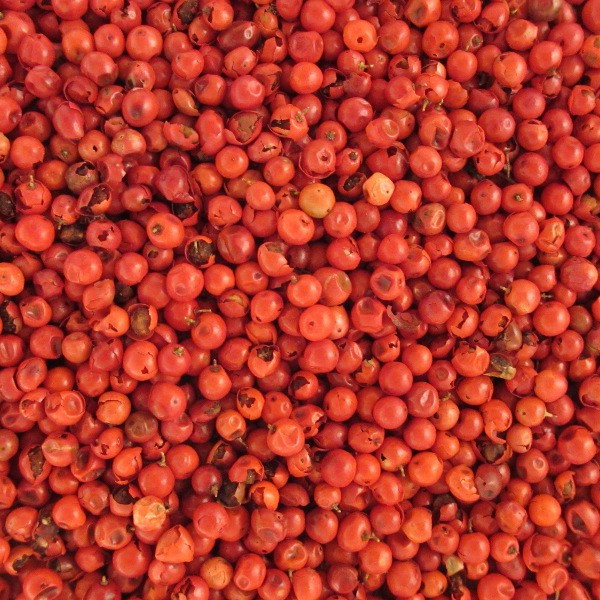
\includegraphics[width=0.33\textwidth]{imgs/spices/pepper-pink-1.jpg}
	\caption{Pink peppercorns (\taxon{Schinus terebenthifolius}).}
	\label{fig:pink_pepper}
\end{wrapfigure}

There are other aromatic, spice yielding plants (other kinds of peppers, if you like) in the \textit{Piperaceae} family, constituting to different species, such as cubebs, tailed peppers, or Java peppers (\taxon{Piper cubeba}), (Indian) long peppers (\taxon{P. longum; P. retrofactum}), ``piper chilies'' (\taxon{P. chaba}), Ashanti/Benin pepper (\textit{P. guineense}), etc., and they will be referred to using these common names throughout. Cubeb, and  long pepper especially, were more common in ancient times but virtually disappeared from the global spice trade in the modern age. Other, less common spices unrelated to the \textit{Piper} genus, such as pink peppercorns from South America (\textit{Schinus molle; S. terebinthifolia}), Sichuan peppers from East Asia (\textit{Zanthoxylum spp.}), and alligator peppers (\taxon{Aframomum danielli}) from Africa are sometimes referred to as ``false peppers''. These will always be referred to with their usual full vernacular names to avoid confusion.
% (America pepper: chili) and peppercorn more to true pepper) explain in the pepper conundrum section.

% Do other peppers at the end of this

According to \textcite[695]{mabberley_mabberleys_2017}, the following common names refer to the species \textit{Piper nigrum}: pepper, black pepper, Madagascar pepper, and white pepper. Except the green peppercorns mentioned above, other spices, such as the Sichuan peppers from China, pink peppercorns from Brazil, and Guinea peppers (\textit{Aframomum melegueta}) from tropical West Africa are different, often botanically unrelated species. Only connected by their names and similar uses, looks, or flavour profiles.




\subsection{The Botany of Black Pepper} 

% ORIGIN:
Pepper is native to the Malabar region in South India where the Western Ghats, a mountain range parallel to the coastline, traps the monsoon rains. This results in the most humid region in India, making it one of the plant biodiversity hot-spots on Earth \autocite[1]{ravindran_black_2000}. Often called the ``king of spices'', pepper originates here in the evergreen tropical forests of Kerala, which is the origin and centre of plant diversity for the ``queen of spices'' as well: cardamom \autocite[1]{ravindran_black_2000}.
Wild populations of pepper and closely related species grow in the moist, shady forests, up to 1200\,m above sea level \autocite{ravindran_piper_2017}. Pepper is cultivated for thousands of years in these areas, and once South India was the only place that produced it. Due to the human desire for this valuable spice, the crop was slowly transplanted from here to other tropical zones, mainly in the Asia-Pacific: Sri Lanka, Malaysia, Indonesia; but also to the West as far as Madagascar and Brazil. Today it is cultivated in 26 countries \autocite{ravindran_black_2000}. The top five producers in 2020 were Vietnam, Brazil, Indonesia, India, and Sri Lanka.\footnote{In order of production quantity, from highest to lowest. All production data is from FAOSTAT (Food and agriculture data of the Statistics Division, Food and Agriculture Organization of the United Nations): \url{https://www.fao.org/faostat/en/\#home}; license: CC BY-NC-SA 3.0 IGO.}
% THE PLANT:
Pepper grows on a perennial vine, blooming a cluster of small flowers on hanging spikes that bring young, round fruits that are first green, turning to bright red as they ripen; resembling berries. Pepper plants in their native habitats spread on the forest floor, or climb over rocks, shrubs, and trees. Pepper prefers the hot tropics with high humidity, and optimal temperatures of around 20-30°C. Open cultivation is possible in places where rainfall is well distributed (e.g.: Thailand, Vietnam, Malaysia), whereas in India shade is required because of the 6 months of drought between monsoon seasons \autocite{ravindran_piper_2017}. Wild pepper species are dioecious\footnote{Bot.: the male and female reproductive organs are found in separate individuals.}, having male and female individuals, while the domesticated pepper populations became monoecious:\footnote{Bot.: having both the male and female reproductive organs in the same individual; hermaphrodite.} one plant is both male and female. This is probably due to thousands of years of selective multiplication and it leads to greater quantities in production: bisexual flowers mean high fruit yields \autocite[38]{ravindran_black_2000}.
% CULTIVATION:
Pepper lianes are propagated from cuttings, and being climbers, they are usually grown around trees for live support, or with the use artificial poles \autocite[216]{van_wyk_culinary_2014}. 

% HARVESTING:
When it comes to harvesting, the techniques are different depending on the intended end product. In the case of black pepper, the near-ripe (still green) fruits are hand-picked and sun-dried in the course of several days up to two weeks. Oxidization leads to the darkening of the pericarp\footnote{Bot.: In fruit anatomy, pericarp is the collective name for the outer layers around the seed of a fleshy fruit or drupe: the endocarp (innermost covering of the seed; the pit), the mesocarp (flesh), and the exocarp (skin).} (the outside skin and flesh of the fruit) to a hue ranging from deep brown to jet black, while also attaining the signature wrinkles and dimples \autocite[254]{hill_contemporary_2004}. The drying process can be sped up by boiling the pepper fruits in hot water for a short time. Chemical changes induced by the heat hasten the subsequent oxidization process, which causes the outer layer to gradually shrivel and blacken while getting dried \autocite[216]{van_wyk_culinary_2014}. White pepper is obtained by letting moisture and micro-organism dissolve the cellular tissue of the fully ripe red fruits, basically letting them rot in a technique called retting\footnote{}. The fruits' decomposed skin and flesh are easily removed by hand or machine after soaking and gentle washing, and the remaining pale seed is then dried on the sun, or bleached \autocite[216]{van_wyk_culinary_2014}. Green peppercorns are a result of traditional pickling, or in modern times rapid freeze-drying of the unripe fruits as a way to prevent fermentation. This process results in a product with a light weight and seemingly higher price. Occasionally the ripe, red fruits are sold as well to be used fresh, but the ``true'' red peppercorns---as \textcite{hill_contemporary_2004} calls them---are rare and mostly found in producing areas: they loose their vigour within days of harvest and so must be used fresh unless preserved in vinegar or brine. As it is a hallmark of spices, the two varieties that are dried (black pepper and white pepper) are much more known worldwide, their dry quality allows them to be transported on longer journeys. If we think of white pepper as de facto decorticated black pepper, we would rightly guess that the flavour of white pepper is weaker than black pepper, as the outer peel of black pepper contains much of the spicy compounds responsible for the heat. Green peppercorns have an even milder taste and a much shorter shelf-life.
%CULTIVARS
Indigenous to the Malabar coast, a well known and popular variant is the Malabar pepper or Malabar black, a commodity sought-after by traders since Roman times \autocite{de_romanis_indo-roman_2020}. Another famous name on the market is the Tellicherry black, which according to spice traders is not a regional designation, but rather a requirement of size. If a peppercorn is larger than 4.25 mm pinhead, it is classified as Tellicherry \autocite{eirinberg_tellicherry_2021}. Other famous and/or protected pepper variants with Geographical Indication (GI) certificates are Kampot pepper from Cambodia, the Muntok white and Sarawak white from Indonesia and Malaysia respectively, and the Penja pepper from Cameroon. A relatively recent publication by pepper grower and merchant \textcite{de_kerros_pepper_2016} accompanied by remarkable photographs aims to present all the dozens of pepper varieties around the world that are available to those with an adventurous taste.
% FLAVOUR COMPOUNDS:
Pepper owes its punch to the alkaloid piperine, while the wrinkly pericarp supplies the complex spicy aroma and flavour thanks to a high number of chemical compounds in the form of volatile oils \autocite[467]{ravindran_black_2000}. The most powerful one of which is rotundone, a highly potent compound also found in Shiraz wines \autocite{wood_wine_2008}. For more on details on the botany, chemistry, cultivation, agronomy, and other aspects of black pepper, please refer to \textcite{ravindran_black_2000, nair_agronomy_2011, parthasarathy_chemistry_2008}.



% HISTORY:
\subsection{The History of Black Pepper}

The history of pepper accompanies the history of mankind from the earliest times of contact and exchange between civilizations. The story of pepper is global and must travel to Ancient Egypt to begin. According to a popular anecdote in books and articles about pepper, peppercorns were used in the embalming process of mummies \autocite{ravindran_black_2000}, and they were found in the nostrils of Ramses II \autocite[168]{turner_spice_2004}. I have read this on many occasions, and I have spend way too much time to find out if this is true or not. In short, I there is no definitive answer, but that the alleged peppercorns were only ``seen'' through X-ray, and that the original reports are dubious at best, as reported by \textcite[206]{bucaille_mummies_1990}. Ramses II died in 1213 \BC{}, and even if these specific are problematic, it is said that peppercorns and cinnamon were imported ``from Southeast Asia and the East Indies'' and thus available to wealthy citizens of Egypt as early as New Kingdom era (\nth{16} c. \BC{}--\nth{11} c. \BC{}) \autocite[394]{salima_diet_2005}.

Pāṇini, the famous Sanskrit grammarian (ca. 4--\nth{6} c. \BC{}) recorded the use of pepper in spiced wine, and pepper appears in early Indian medical texts of Suśruta as well \autocite{ravindran_black_2000}. In the \nth{4} century, Theophrastus recorded and described both black pepper and long pepper, and by the \nth{1} century \AD{} its source was accurately describe by Pliny the Elder; stating that black pepper is from south, long pepper is from north India. Rome conquered Egypt in 30 \BC, and with that the pepper trade as well, which was a key enterprise in Rome's later financial success. From here onwards, the history of pepper within the Indo-Roman trade is well studied and documented, for further details please see \textcite{sidebotham_berenike_2011,de_romanis_indo-roman_2020,miller_spice_1969}. 

% Peppercorn in fist century as far as Germany (Czarra)

During the late Middle Ages, pepper also brought great riches to Europe, the former wealth of Venice was due to its trade. After the crusades, European sea powers tried to get ahold on the monopoly of the spice trade, and Vasco de Gama's landing near Calicut in 1498 in the Venetian, Portuguese, Spanish, Dutch, and English vied with each other for centuries up to the modern era. The story of pepper is very well explored in the Age of Exploration as well, there is no need for me to delve into it deeper. I recommend \textcite{shaffer_pepper_2013} for those interested in the big picture, but the sections about pepper in \textcite{dalby_dangerous_2000,turner_spice_2004} are also well researched.

% Pepper reached Southeast Asia probably during the times?

% A Chinese envoy visited the Malabar coast in search of pepper. 4th c. BC? Who

% TIMELINE IN RAVINDRAN
% Originally black pepper was a forest produce
% Black pepper was essentially a forest produce in the past, people collected it from
% forests, where it abounded. The collected pepper was brought to local markets for
% retail trade with Arab merchants. Domestication of pepper appears to be a much later
% event. There is, only speculative evidence as to when pepper was introduced to other
% countries as a domesticated crop. Colonists from India are believed to have introduced
% pepper cultivation to Indonesia about 100 B.C. (Rosengarten 1973). Many such
% introductions surely might have taken place subsequently also. The landmarks in the
% colourful history of pepper are given below. Ravindran 2000 

% \autocite{pegolotti_pratica_1936}

% Wyk:
% Pepper featured prominently in the
% ancient world and was a source of fabulous wealth
% during the medieval and colonial spice trade. The
% Dutch and Afrikaans expression “peperduur”
% reflects the high price it once had. Pepper provided
% the pungency (“pep”) of Indian food until it was
% partially replaced by chilli peppers from the New
% World. It nevertheless remains the most important
% and popular of all spices in terms of overall value
% and trade volume.

% Black pepper is the most important and widely used spice. Black pepper (hereafter mentioned simply as pepper) is valued for its characteristic pungency and flavour. It has been used extensively from ancient times as a spice and condiment in a variety of food preparations. Pepper is famous as a traditional medicine; it is also famous as a home remedy. Globally, pepper accounts for 34\% of the total spices traded. In all countries pepper is used for flavouring food and for preserving processed foods. Pepper played a very significant role in shaping the history of mankind. It was the first oriental spice to reach the Western world. The European nations vied with each other to get the monopoly over the spice trade and hegemony over the spice-producing countries of the East that eventually led to the discovery of a sea route to India by Vasco da Gama. This event changed the history of the world radically in the centuries that followed. ENCYCL

% Among the spices, black pepper is the king. It is the most important, the most
% popular and the most widely used spice in the world. It has extensive culinary uses
% for flavoring and preserving processed foods and is also important medicinally. Of
% the total spices traded internationally, pepper accounts for about 34 % (throughout
% this chapter, pepper is used to mean black pepper, unless otherwise stated). South
% West India, particularly the Western Ghats regions of the South India, is the centre
% of origin of this important spice. Black pepper was the fi rst oriental spice to be
% introduced into the Western world, and it was well known among the Romans and
% Greeks. In the Middle Ages, pepper, assumed great importance in Europe. Its use
% resulted in revolutionary changes in western cooking. For a comprehensive treatment
% of black pepper, the reader may consult Ravindran (2000a) and Ravindran
% et al. (2006). Bezerra et al. recently (2009) summarized the various aspects of black

\subsection{The Names of Black Pepper}

\subsubsection{English}

\begin{etymology}\label{ety:pepper}
English \textit{pepper}
<\textss{?} West Germanic* \textit{*pipor} `id.'
< Latin \textit{piper} `black pepper, long pepper'
< Ancient Greek {πέπερι} \textit{péperi} `id.'
< Middle Indo-Aryan* {पिप्परी } \textit{pipparī} `long pepper'
< Sanskrit {पिप्पलि } \textit{pippali} `long pepper \textit{Piper longum} (plant and berry); a berry'\footnote{\textcite{oed; med; bosworth_anglo-saxon_2014}; \textcite{oe}; \textcite{lewis_latin_1879}; \textcite{liddell_greek-english_1940}; \textcite[599]{sheth_paia-sadda-mahannavo_1923}; \textcite[626]{monier-williams_sanskrit-english_1899}}
\end{etymology}

The word \textit{pepper} arrived to modern English via Middle English \textit{peper} and Old English \textit{pipor, piper}, from an early, Proto-West Germanic borrowing of Latin \textit{piper}.\footcite[pepper]{oed} The Latin word comes from Greek \gr{πέπερι} \textit{péperi}, a word ``of oriental origin''\footcite[pepper]{hoad_concise_2003} or ``Indic origin''.\footcite[pepper]{ahd} The source is most probably from a Middle Indo-Aryan language, akin to Prakrit \textit{pipparī}\footcite[599]{sheth_paia-sadda-mahannavo_1923}, probably via Pahlavi (Middle Persian)\footcite[pepper]{oe}, ultimately from Sanskrit \textit{pippali} or \textit{pippalī}.\footcite[628 \link{https://www.sanskrit-lexicon.uni-koeln.de/scans/MWScan/2014/web/webtc/servepdf.php?page=0628}]{monier-williams_sanskrit-english_1899}

As for the meaning, we know that in Latin the word \textit{piper} was used for both black pepper and long pepper, and this is true for the Greek word as well. As long pepper gradually disappeared and was completely replaced by black pepper in the Middle Ages, so vaned the that sense of the word. The original word's meaning however was exclusively long pepper, \textit{pippali} did not refer to black pepper. In \textcite{monier-williams_sanskrit-english_1899}, \textit{pippali} is `long pepper', while \textit{pippalī} refers to `a berry; Piper longum (both plant and berry)'. The Sanskrit word for `black pepper' was \sa{मरिच} \textit{marica}\footcite[790]{monier-williams_sanskrit-english_1899}, attested in the \gls{Sushruta}, the foundational text of \gls{Ayurveda}. Hindi-Urdu \sa{मिर्च}/\fa{مرچ} \textit{mirch} is the most obvious descendant of the Sanskrit word, and it is similar in meanings to the word \textit{pepper} in English today: by itself it rather refers to chili, while with a distinguishing word, it refers to black pepper (i.e. \textit{kālī mirc} [black pepper]). The use of both black and long pepper in India can be dated to ancient times, as Ayurvedic texts compiled in Sanskrit, such as the \gls{Sushruta} testify. Together with ginger (\textit{śṛṅgavera} in Sanskrit), these three spices are a base combination in traditional Indian medicine, the name for which is \sa{त्रिकटु} \textit{trikaṭu} `three spices'.

The ancestors of English speakers adopted the word during the Anglo-Saxon period, before they arrived to England, and so its cognates are found in other West Germanic languages as well.\footcite[pepper]{cresswell_oxford_2021} 

% Cognates:  Old Saxon \textit{pipari}, \textit{pepar} (Dutch \textit{peper}, Scots pepar), Old High German \textit{pfeffar} (German \textit{Pfeffer}), Old Norse \textit{piparr} (Danish \textit{peber}, Swedish \textit{peppar}, Icelandic \textit{pipar}).

% Leaves of P. sarmentosum are the cha plu of Thai cuisine and those of P. auritum the hoja santa of Mexican cuisine. Plus Piper betle = betel? no.

The term \textit{peppercorn} is a compound of \textit{pepper} and \textit{corn}, in its previous sense `grain', and it is used to refer to a single piece of the pepper fruits. Many other names of black pepper actually refer to varieties and cultivars, e.g., \textit{Malabar pepper}, \textit{Kampot pepper}, and the above-mentioned Tellicherry black.

\begin{table}[!ht]
\centering
\begin{tabularx}{\textwidth}{@{}l>{\itshape \small}lL>{\small}l@{}}
\toprule
\textbf{\#} & \multicolumn{1}{l}{\textbf{Species}} & \multicolumn{1}{l}{\textbf{Name}} & \multicolumn{1}{l}{\textbf{Source}} \\
\midrule
1	& Piper nigrum	& black pepper	& \textcite{van_wyk_culinary_2014} \\
2	& Piper nigrum	& green pepper	& \textcite{oed} \\
\textbf{3}	& \textbf{Piper nigrum}	& \textbf{pepper}	& \textbf{\textcite{van_wyk_culinary_2014}} \\
4	& Piper nigrum	& peppercorn	& \textcite{oed} \\
5	& Piper nigrum	& white pepper	& \textcite{oed} \\
\bottomrule
\end{tabularx}
\caption{Various names for pepper in English.}
\label{table:names_pepper_en}
\end{table}



\subsubsection{Arabic}

\begin{etymology}\label{ety:fulful}
Arabic {فلفل} \textit{filfil, fulful} `pepper'
< Persian {پلپل} \textit{pilpil} `id.'; cf. cognates Old Armenian \hy{պղպեղ} \textit{płpeł}, Old Georgian \ka{პილპილი} \textit{ṗilṗili}
<\textss{?} Middle Indo-Aryan \textit{?} `long pepper'
< Sanskrit {पिप्पलि } \textit{pippali} `long pepper \textit{Piper longum} (plant and berry); a berry'\footnote{\textcite[2434]{lane_arabic-english_1863}; \textcite{sq}}
\end{etymology}

Arabic \textit{fulful}\footnote{``also pronounced \textit{filfil} but the vulgar pronounce it [thus] with \textit{kesr}---name of the /i/---and the pronouncing it with \textit{kesr} is said to be not allowable [...]'', as reported by \textcite[2434]{lane_arabic-english_1863}} comes via Persian from essentially the same Indic etymon as English pepper: Sanskrit \textit{pippali}. The word is first attested Arabic spice term in this set (\AD \nth{6} century). Similarly to almost all other languages, the word can be appended by the adjectives for black and white. And, as \textit{fulful} is a ``collective'' term, we can refer to a singular peppercorn by adding the singular feminine marker \textit{-a} (t\={a} marb\={u}ta) suffix.

\begin{table}[!ht]
\centering
\begin{tabularx}{\textwidth}{@{}l>{\itshape \small}lr>{\itshape}lL>{\small}l@{}}
\toprule
\textbf{\#} & \multicolumn{1}{l}{\textbf{Species}} & \multicolumn{1}{l}{\textbf{Name}} & \multicolumn{1}{l}{\textbf{Tr.}} & \multicolumn{1}{l}{\textbf{Gloss}} & \multicolumn{1}{l}{\textbf{Source}} \\
\midrule
\textbf{1}	& \textbf{Piper nigrum}	& \textbf{فلفل}	& \textbf{fulful}	& \textbf{pepper}	& \textbf{\textcite{wehr_dictionary_1976}} \\
2	& Piper nigrum	& فلفل أبيض	& fulful abyaḍ	& white pepper	& \textcite{baalbaki_-mawrid_1995} \\
3	& Piper nigrum	& فلفل أسود	& fulful aswad	& black pepper	& \textcite{baalbaki_-mawrid_1995} \\
4	& Piper nigrum	& فلفلة	& fulfula	& peppercorn	& \textcite{wehr_dictionary_1976} \\
\bottomrule
\end{tabularx}
\caption{Various names for pepper in Arabic.}
\label{table:names_pepper_ar}
\end{table}



\subsubsection{Chinese}

\begin{etymology}\label{ety:hujiao}
\textbf{Mandarin Chinese} {胡椒} \textit{hú​jiāo} `black pepper' [barbarian-pepper], from 胡 \textit{hú​} `Western barbarians, steppe nomads' + 椒 \textit{jiāo} `pepper, spice' (\textit{jiāo} was the prototype spice in China, originally referring to the local ``Sichuan pepper'' which is now called 花椒 \textit{huājiāo} [flower-pepper]), [Northern and Southern] 420-445\footnote{\textcite{schuessler_abc_2007}}
\end{etymology}

There is no surprise in the anatomy of pepper terms in Chinese neither, except that there we have an extra layer of modifiers, namely \textit{hu} `Western barbarians, steppe nomads'. This indicates two things. One, black pepper must have arrived China from the west, transmitted by the nomadic peoples of the steppe outside of Chinese territories. Two, \textit{jiao}, the term now denoting all kinds of `peppers' existed before \textit{Piper nigrum} was known, and it refers to the prototype spice item for Chinese speakers. With some background knowledge, we know that this prototype spice in China were the fruits of \textit{Zanthoxylum} species, otherwise known as Sichuan peppers. \textit{Hujiao} `black pepper' first appeared in the \gls{Hou Hanshu} ca. \AD 450.

\begin{table}[!ht]
\centering
\begin{tabularx}{\textwidth}{@{}l>{\itshape \small}ll>{\itshape}lL>{\small}l@{}}
\toprule
\textbf{\#} & \multicolumn{1}{l}{\textbf{Species}} & \multicolumn{1}{l}{\textbf{Name}} & \multicolumn{1}{l}{\textbf{Tr.}} & \multicolumn{1}{l}{\textbf{Gloss}} & \multicolumn{1}{l}{\textbf{Source}} \\
\midrule
1	& Piper nigrum	& \tradchinesefont{白胡椒}	& báihújiāo	& white-barbarian-pepper	& \textcite{mdbg} \\
\textbf{2}	& \textbf{Piper nigrum}	& \textbf{\tradchinesefont{胡椒}}	& \textbf{hújiāo}	& \textbf{barbarian-pepper}	& \textbf{\textcite{hu_food_2005}} \\
3	& Piper nigrum	& \tradchinesefont{黑胡椒}	& hēihújiāo	& black-barbarian-pepper	& \textcite{mdbg} \\
4	& Piper nigrum	& \tradchinesefont{綠胡椒}	& lǜhújiāo	& green-barbarian-pepper	& \textcite{regency_spices_regency_2022} \\
5	& Piper nigrum	& \tradchinesefont{青胡椒}	& qīnghújiāo	& green-barbarian-pepper	& \textcite{regency_spices_regency_2022} \\
\bottomrule
\end{tabularx}
\caption{Various names for pepper in Chinese.}
\label{table:names_pepper_zh}
\end{table}



\subsubsection{Summary}

\begin{table}[!ht]
\centering
\begin{tabularx}{\textwidth}{@{}ll>{\itshape}lLl>{\small}l@{}}
\toprule
\textbf{\#} & \textbf{Language} & \multicolumn{1}{l}{\textbf{Term}} & \textbf{Gloss} & \textbf{Loan} & \multicolumn{1}{l}{\textbf{Source}} \\
\midrule
1	& English	& black pepper	& 	& maybe	& \textcite{oed} \\
2	& English	& pepper	& 	& yes	& \textcite{oed} \\
3	& English	& white pepper	& 	& maybe	& \textcite{oed} \\
\midrule
1	& Arabic	& fulful	& pepper	& yes	& \textcite{wehr_dictionary_1976} \\
2	& Arabic	& fulful abyaḍ	& white pepper	& no	& \textcite{baalbaki_-mawrid_1995} \\
3	& Arabic	& fulful aswad	& black pepper	& no	& \textcite{baalbaki_-mawrid_1995} \\
4	& Arabic	& fulfula	& peppercorn	& no	& \textcite{wehr_dictionary_1976} \\
\midrule
1	& Chinese	& báihújiāo	& white-barbarian-pepper	& no	& \textcite{mdbg} \\
2	& Chinese	& hújiāo	& barbarian-pepper	& no	& \textcite{defrancis_abc_2003} \\
3	& Chinese	& hēihújiāo	& black-barbarian-pepper	& no	& \textcite{mdbg} \\
\bottomrule
\end{tabularx}
\caption{Conventionalized names for pepper in English, Arabic, and Chinese, found in dictionaries.}
\label{table:names_pepper}
\end{table}



% \begin{figure}[!hbt]
%     \centering
%     \includegraphics[width=\linewidth]{imgs/pepper.pdf}
%     \caption{Etymology of the English word \textit{pepper}, and an illustration of its approximate route.}
%     \label{map:pepper_etymology}
% \end{figure}










% EE: The Concise Oxford Dictionary of English Etymology:
% OE. piper, -or = OS. pipari, pepar (Du. peper), OHG. pfeffar (G. pfeffer); WGmc. — L. piper — Gr. péperi, of oriental orig.; cf. Skr. pippalī́t berry, peppercorn.

% OE: 
% pepper (n.)
% "dried berries of the pepper plant," Middle English peper, from Old English pipor, from an early West Germanic borrowing of Latin piper "pepper," from Greek piperi, probably (via Persian) from Middle Indic pippari, from Sanskrit pippali "long pepper." The Latin word is the source of German Pfeffer, Italian pepe, French poivre, Old Church Slavonic pipru, Lithuanian pipiras, Old Irish piobhar, Welsh pybyr, etc.
% Application to fruits of the Capsicum family (unrelated, originally native of tropical America) is from 16c. To have pepper in the nose in Middle English was "to be supercilious or unapproachable."
% pepper (v.)
% "to sprinkle as with pepper," 1610s, from pepper (n.). Old English had gepipera. Meaning "to pelt with shot, etc.; hit with what pains or annoys" is from 1640s. Related: Peppered; peppering.

% MW:
% Middle English peper, from Old English pipor; akin to Old High German pfeffar pepper, Old Norse piparr; all from a prehistoric Germanic word borrowed from Latin piper pepper, from Greek peperi, probably from Sanskrit pippali long pepper
% First Known Use: before 12th century (sense 1a)

% AH:
% [Middle English peper, from Old English pipor, from Latin piper, long pepper, black pepper, from Greek peperi, of Indic origin; akin to Prakrit pipparī, long pepper, from Sanskrit pippalī, from pippalam, berry, fruit of the pipal tree, of unknown origin.]

% WK:
% From Middle English peper, piper, from Old English piper, from Proto-West Germanic *piper, from Latin piper, from an Indo-Aryan source; compare Sanskrit पिप्पलि (pippali, “long pepper”). The name was given to the capsicum fruit because of its unusual spicy taste, not unlike the European spice.

% Wo: The Oxford Dictionary of Word Origins:
% The Anglo-Saxons adopted the word for this highly prized spice before they invaded England, for it is found in other West Germanic languages. The word came via Latin from Greek peperi, from Sanskrit pippalī ‘berry, peppercorn’. 
%The phrase peppercorn rent is from the once-common practice of stipulating the payment of a peppercorn as a nominal rent. (true?)
% Cognate with Scots pepar, Saterland Frisian Pieper, West Frisian piper, Dutch peper, German Low German Peper, German Pfeffer, Danish peber, Swedish peppar, Icelandic pipar. Doublet of peepul. 



% The pepper conundrum:

% Before we delve into the chaos of \textit{pepper-linguistics}, we should make the botany and geography absolutely clear. There are essentially three major sources of edibles we can refer to as peppers: (1) \textit{Piper}, a pantropical\footnote{??} genus known for black and white pepper, long pepper, and cubeb pepper from South and South East Asia; (2) \textit{Capsicum}, the genus of both hot chile and mild bell pepper species and their numerous cultivars native to the Americas; and (3) \textit{Zanthoxylum}, a vast and cosmopolitan\footnote{??} genus of various species yielding Sichuan peppers favoured in East Asia. There are many more aromatic products denoted with the name \textit{pepper} in English, but for our task focusing on the above three genera is sufficient. Also, the majority of globally relevant ``peppers'' belong to these groups as well. Nevertheless, for a full paragraph of a detailed list of plants, please see \textcite[695]{mabberley_mabberleys_2017}.

% pepper Piper nigrum; African p. Xylopia aethiopica; Ashanti or Benin p. P. guineense; bell p. Capsicum annuum Grossum Group; p.berry Drimys spp.; betel p. P. betle; bird p. C. a.var.glabriusculum; black p. P. nigrum; bush p. Clethra alnifolia; cayenne p. Capsicum annuum Longum Group; cherry p. C. a. Cerasiforme Group; chilli p. C. a.Longum Group; Chinese p. Zanthoxylum simulans; cone p. C. a. Conoides Group; p.corns, pink or red Schinus terebinthifolius; Ethiopian p. X. aethiopica; green p. C. a. Grossum Group; Guinea p. Aframomum melegueta, X. aethiopica; Indian long p. P. longum; Jamaican p. Pimenta dioica; Japanese p. Z. piperitum; Java p. Piper cubeba; Kawa p. P. methysticum; long p. P. longum; Madagascar p. P. nigrum; malagueta or melegueta p. A. melegueta; negro p. X. aethiopica; red or sweet p. C. a. Grossum Group; Saturday-night p. Euphorbia helioscopia; Sichuan p. Z. simulans; p. tree S. molle, Kirkia wilmsii, P. excelsum; wall p. Sedum acre; water p. Persicaria hydropiper; W African black p. Piper clusii; white p. P. nigrum

% Pepper in English

% ...


% The confusion of the two kinds of pepper---most notably of black pepper and chile pepper in English---is also present in Chinese, as well Arabic. Whether in culinary or medicinal spice terminology, or just in vernacular names in daily conversation, the curse of ``one word for all peppers'' is present in many languages.




% Pre-Qin and Han -> Ancient Classics -> Book of Poetry -> Lessons from the states -> Odes Of Tang -> Jiao Liao

% Transl. James Legge
% https://ctext.org/book-of-poetry/jiao-liao?searchu=%E6%A4%92%E8%81%8A%E4%B9%8B%E5%AF%A6%E3%80%81%E8%95%83%E8%A1%8D%E7%9B%88%E5%8D%87%E3%80%82&searchmode=showall#result
% \url{https://en.wikipedia.org/wiki/Classic_of_Poetry}

% Our assumption will only strengthen if we search the word history of black pepper, a native of India. It first appears in
% https://ctext.org/pre-qin-and-han?searchu=%E8%83%A1%E6%A4%92

% Pre-Qin and Han


% The first occurrence of \textit{hujiao}

% The origin of hujiao `black pepper' in Chinese






% \begin{figure}
% \label{fig:pepper}
% \begin{forest}
% for tree={grow'=0,calign=center,font=\footnotesize, s sep=1,inner sep=1,outer sep=1},
% forked edges,
% [Sanskrit\\pippali
%     [Ardhamagadhi Prakrit\\pipparī [Awadhi\\pīpri]]
%     [Gandhari [Middle Iranian\\\textrightarrow [Persian\\pelpel [Arabic\\\textrightarrow filfil [Persian\\\textrightarrow felfel]] [(Arabic)\\\textrightarrow falāfil] [Baluchi\\\textrightarrow pilpil] [Hebrew\\\textrightarrow pilpel] [Swahili\\\textrightarrow pilipili] ] [Old Armenian\\\textrightarrow płpeł [Armenian\\\textrightarrow płpeł]] [Old Georgian\\\textrightarrow ṗilṗili [Georgian\\ṗilṗili]] ]]
%     [Pali\\pipphalī]
%     [Magadhi Prakrit [Assamese\\pipoli] [Bengali\\pipul] [Bhojpuri\\pīpri]]
%     [Maharastri Prakrit [Old Marathi\\piṃpaḷī [Marathi\\pimpḷī]] [Kannada\\\textrightarrow hippali]]
%     [Sauraseni\\Prakrit [Nepali\\piplā] [Gujarati\\pīpar] [Hindustani [Hindi\\pīpal; pīpar] [Urdu\\pīpal] [(English)\\\textrightarrow peepul]] [Punjabi\\pippalī] [Ancient Greek\\\textrightarrow péperi* [Greek\\pipéri [Ottoman\\Turkish\\biber [Turkish\\biber [Armenian\\bibar] [Azerbaijani\\bibər] [Crimean Tatar\\biber] [Macedonian\\biber] [Serbo-Croatian\\biber]]] [Aromanian\\piper]] [Latin\\\textrightarrow piper [Basque\\\textrightarrow piperra] [Middle Irish\\pipur [Irish\\piobar] [Manx\\pibbyr] [Scottish Gaelic\\peabar; piobar] [Old Norse\\piparr [Icelandic\\pipar] [Faroese\\pipar] [Norwegian\\pepar] [Swedish\\peparr [Finnish\\\textrightarrow pippuri [Northern Saami\\bihppor]]]] ] [Dalmatian\\pepro] [Italian\\pepe] [Old French\\poivre [French\\poivre]] [Aragonese;\\Catalan;\\Occitan\\pebre]]]]
%     [Old Tamil\\\textrightarrow [Tamil\\tippili] [Malayalam\\\textrightarrow tippali]]
%     [Telugu\\\textrightarrow pippali]
%     [Thai\\\textrightarrow dii-bplii]
%     [Tibetan\\\textrightarrow pi pi ling]
%     [Middle Chinese\\\textrightarrow MC piɪt̚ bʉɐt̚ [Chinese\\bìbá [Japanese\\\textrightarrow hihatsu] [Korean\\\textrightarrow pilbal]]]
% ]
% \end{forest}
% \caption{Caption}
% \end{figure}
















% \small{aguttam, akuttam, alar, alarkay, alarkaycceti, alarmancal,
% alivaliyanmani, amiram, anam, apanam, apayam,
% aricam, aricu, aricuvai, arisu, arittam, arunapakam, arutam,
% aruttakam, aruttam, aruttan, arutti, atittam, aucatikam,
% autatalakamilaku, ayilakikam, bikran, cakankam,
% canucam, canucam, canukam, carapantam, carumapantam,
% catalam, catalamilaku, cattu-molagoi, cavi, cavviyam, cavviyapalam,
% cavyam, celavikacceti, celaviyam, cevviyam,
% ceytakar, chocamirch, cirovikam, ciroviruttam, citamaricam,
% citamarucam, citamarucu, citamarukam, cullituvan,
% cunam, cuppiramaniyam, cur, dhanwantari, dharmapattana,
% dharmavarttana, dolo maricho, eddemunchi, eddemunci,
% fiffile-asvad, fifile-asvad, fifile-gird, filfil aswad, filfil-esiyah,
% filfil siah, filfile-gird, filfile-siyah, filfilgird, filful
% aswad, filfilsiya, filfiluswud, gol mirc, gol-mirch, golmirch,
% golmorich, gulmirch, habush, hapusha, impikam, impilam,
% irambivam, irampikam, irampilam, irampivam, itukam, itukamilaku,
% ivainakitam, ivanattam, jalook, jaluk, kaalimirch,
% kaalu menasu, kadu menasu, kali mirch, kalimirc, kalimirch,
% kalamiri, kalappakacceti, kalappakam, kali mirch, kalimirch,
% kalimirich, kalinai, kalinaikkollu, kalinaimilaku, kalinkam,
% kallinai, kami, kamicakam, kanakam, kanattai, kandanaguli,
% kankola, kantanakuli, kantankuli, kaphavirodhi,
% karam, karee menasu, kari, karikkay, karimenasu, karunelli,
% karutturupayan, karyam, katti, kattirican, katu, katuka, kay,
% kayam, kevakatiraviyam, kevalatiraviyam, kirantikantikam,
% kirusnam, kiruttinam, kola, kolai, kolagam, kolaka, kolakam,
% kolam, kolicam, kolikacceti, krishnam, krishnamushana,
% krsna, kuru-milagu, kuru-mulaka, kurumilagu, kurumilaku,
% kurumulagu, kurumulaka, kurumulaku, maarichamu, maciyam,
% maikkurotikam, maiyi, makaracitakaram, malaittirukkal,
% malaivacapancam, malaiyalam, malaiyali, malaiyaracan,
% malaiyavikam, maliyavikacceti, malaiyinmunivan, malina,
% marica, marica-valli, maricam, maricamu, maricha, maricham,
% marichamu, marichi, marichipatra, marici, marisam,
% mariyal, maruci, marukkam, matankan, meervaela, mellaghoo,
% menasina balli, menasinaballi, menasinakaalu, menasinakalu,
% menasu, mensukaai, milagu, milagu-valli, milaku,
% milakucceti, milakuvalli, mir vel, mirc, mirch, mirch siah,
% mire, mireem, miremu, miri, miricam, miricanam, mirici,
% mirim, miriyaalathige, miriyaalu, miriyal, miriyala-tige,
% miriyalakam, miriyalatige, miriyalu, miriyamu, miriyarkoti,
% miryala-tige, miryalatige, molago-codi, molagacodi, moloovookodi,
% mrishta, mulaku, mulaku koti, mulakukoti, mulatti,
% munchi, munci, muntan, mupparitam, mupparitamilaku,
% murialtiga, musanam, mutanam, nakarenu, nallamilaku,
% nalmilaku, nattumilaku, neriyal, nettakam, nettam, nitiyam,
% olle menasu, ollemenasinaballi, ollemenasu, ollimonasu,
% ooshnam, palini, paluk, paluka, parici, pattuvanestam, pavita,
% pavitam, pilpil, piramamaricam, piramaparicam, pittam,
% pokhlem-mirim, pulipacitam, repam, ruksha, sabe-ricke,
% safedmirch, sarvahita, savyamu, shakanga, shevium, shirovritta,
% shivika, shudha, shyama, siyah mirch, suvrtta, tarapattanam,
% tarmapattanam, tarumapittam, tattuvacam, tavalam,
% tavalamilaku, thinghmarcha, ticcanam, tikshna, tiksna,
% tiraipokki, tirankal, tirankalam, tirankam, tirankanal, tirkuta,
% titcanam, tuvinam, ucakam, ucanam, uciram, usakam, usana,
% usanaka, usanam, ushanam, utanam, uttanam, vacampu,
% vacankiyam, vacikam, vacitam, vallacam, vallicam, vallija,
% vallijam, vallikacceti, valliyam, vara, varishtha, vatamarukkinron,
% vatanacani, vellaiccatikam, vellaiccatikamilaku,
% vellaimilaku, vellaja, vellajam, vellija, venkakkiyam, venkakkiyamilaku,
% venmilaku, venticam, venticamilaku, venuja,
% venuka, venunam, villajam, virani, viruttapalam, viruttapam,
% volloymenasu, vrittaphala, wollemenasu, yavanappiriyam,
% yavanapriya, yavaneshtha, yeddemunci, zira siyah}